\section{Results}
\label{sec:results}
% TODO: Mention the hypopthesis in Results section
This section presents the results of simulations meant to determine the performance of the search algorithms. All benchmarks were run on three maps, an empty map, a simple map, and a complex map. \Cref{fig:bench-maps} shows the three maps, with differing denseness of obstacles, used during testing.

This section presents a comparative evaluation of the developed search algorithms in terms of two key metrics: map coverage over time and computational expense. These metrics are analyzed across environments of varying difficulty. 
Additionally, the consistency between the two simulation environments—\texttt{simple\_sim} and the Gazebo ROS 2 setup—is evaluated to confirm the robustness and portability of the behavior implementations.


\subsection{Simulator Consistency}
A central goal of the dual-simulator framework is to ensure that algorithms implemented using the \texttt{botbrain} interface yield consistent behavior across both simulators. While Gazebo includes more realistic physics and non-deterministic behavior due to its time step and sensor noise, consistency in qualitative behavior (e.g., coverage trend) is still expected.


\subsubsection{Basic Movement}
To verify basic motion consistency, a simple circular movement behavior was executed in both simulators. As shown in \cref{fig:movement-consistency}, the resulting paths are visually similar, indicating that the velocity commands are interpreted similarly in both environments.

In the Gazebo simulation, the path deviates slightly from a perfect circle. This deviation is attributed to realistic physical effects such as wheel slippage and friction between the wheels and the ground. In contrast, the \texttt{simple\_sim} simulator assumes ideal motion without any loss due to slippage or friction, resulting in a more precise circular trajectory.\\


\begin{figure}[H]
  \centering
  \begin{subfigure}[b]{0.45\textwidth}
    \centering
    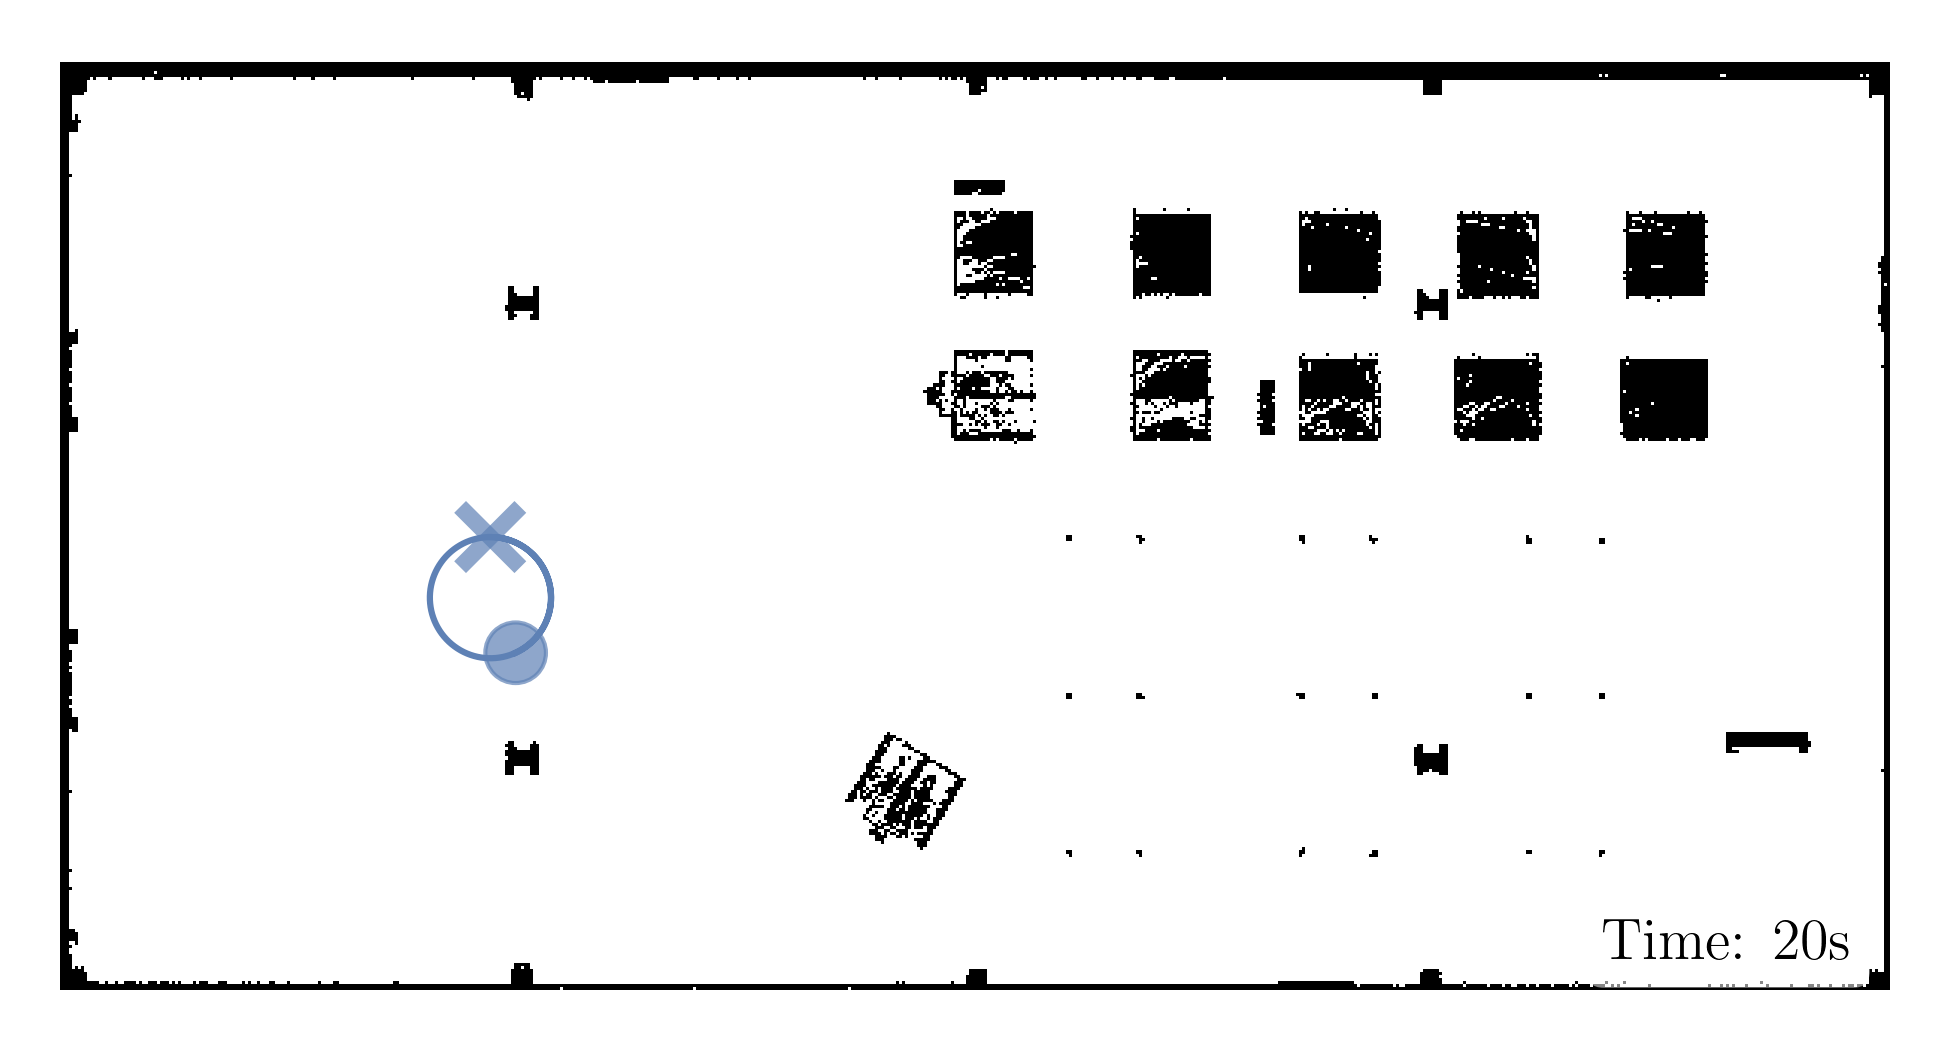
\includegraphics[width=\textwidth]{./figures/plots/consistency/simple-sim-paths-(after-20s).png}
    \caption{Simple Sim}
  \end{subfigure}
  \begin{subfigure}[b]{0.45\textwidth}
    \centering
    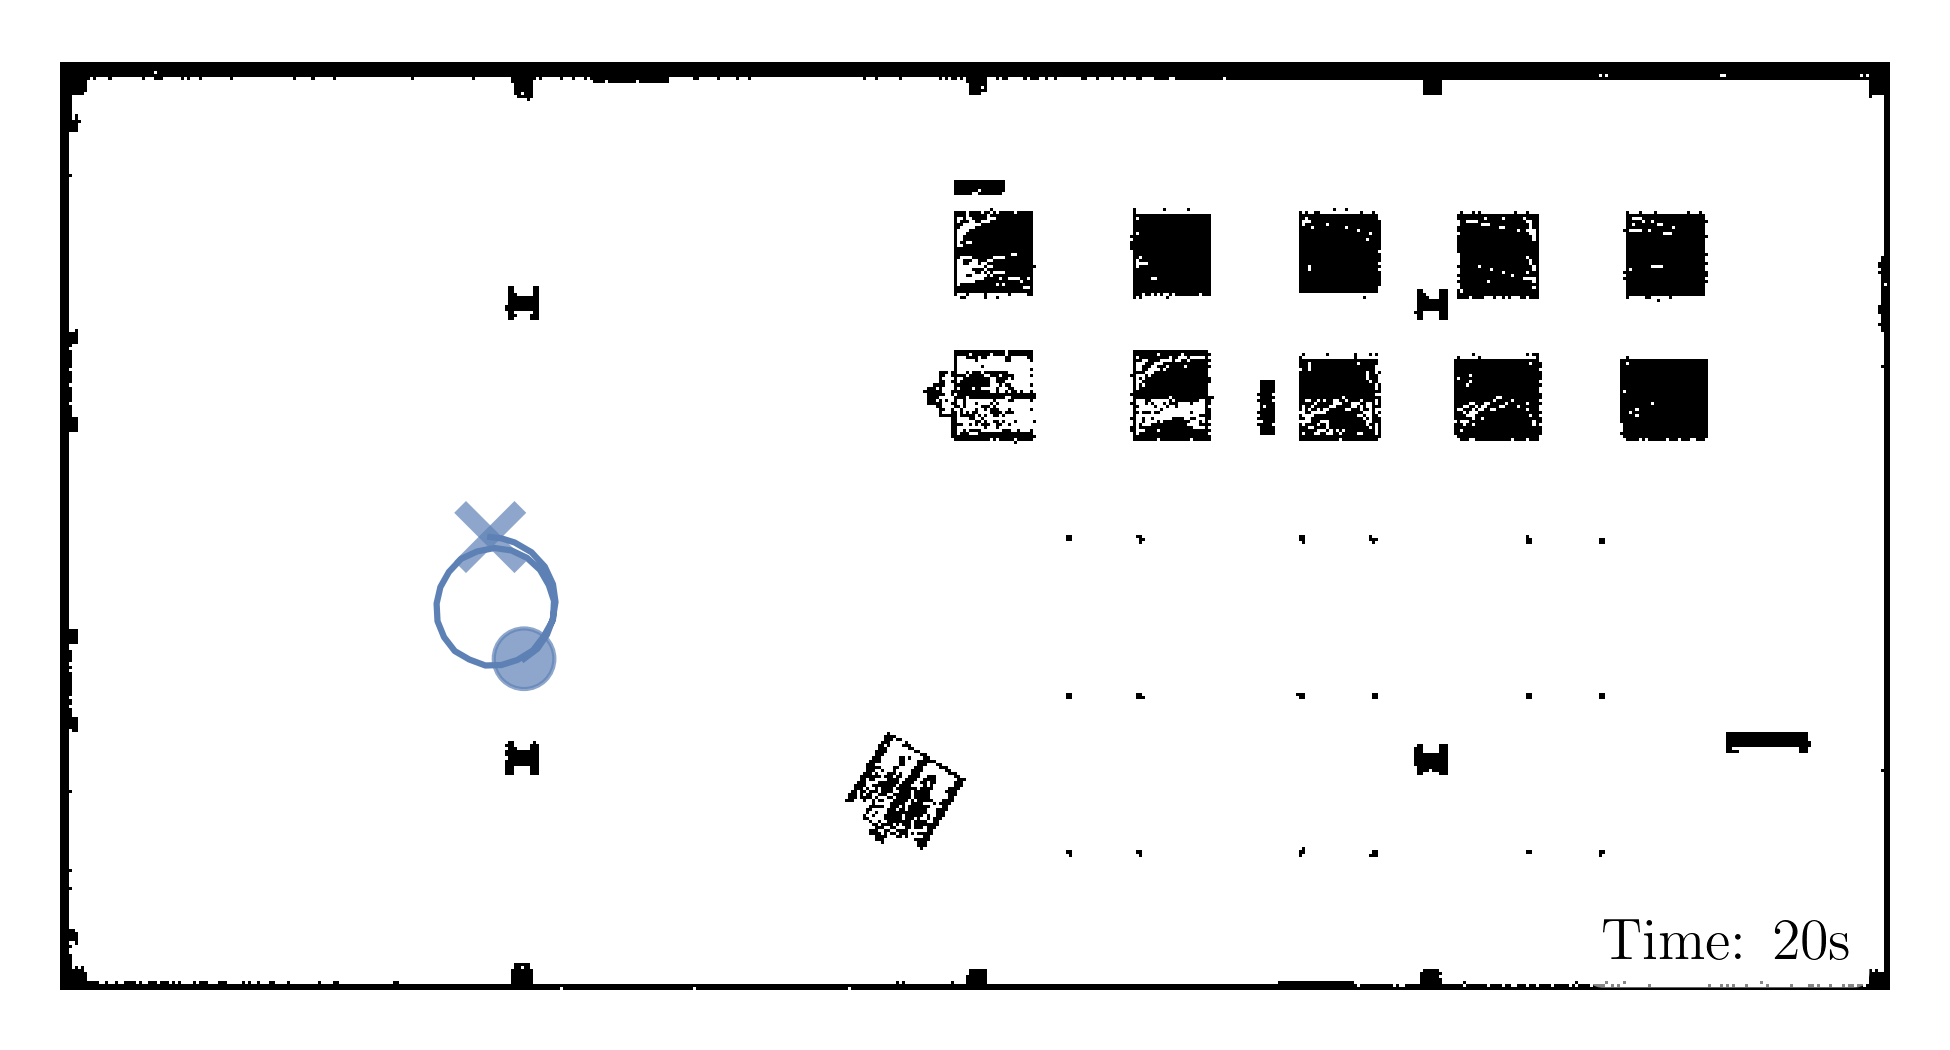
\includegraphics[width=\textwidth]{./figures/plots/consistency/ros-2-paths-(after-20s).png}
    \caption{ROS 2 Gazebo}
  \end{subfigure}
  \caption{Paths produced by a circular behavior in \texttt{simple\_sim} and ROS 2 Gazebo.}
  \label{fig:movement-consistency}
\end{figure}

\subsubsection{Pathing}
% FIX: Change this text
A more complex evaluation was performed by comparing the main search behaviors. 
As shown in \cref{fig:coverage-benchmark-all}, the coverage curves produced by each simulator are closely aligned, particularly in early and mid-stage exploration. 
Minor deviations are attributed to non-determinism in Gazebo and slight differences in physics and sensor modeling.

The expectation is that the differences in the Gazebo and \texttt{simple\_sim} coverage over time, see \cref{fig:coverage-benchmark-diff}, will be consistent between the different search behaviors.

\begin{figure}
    \begin{center}
        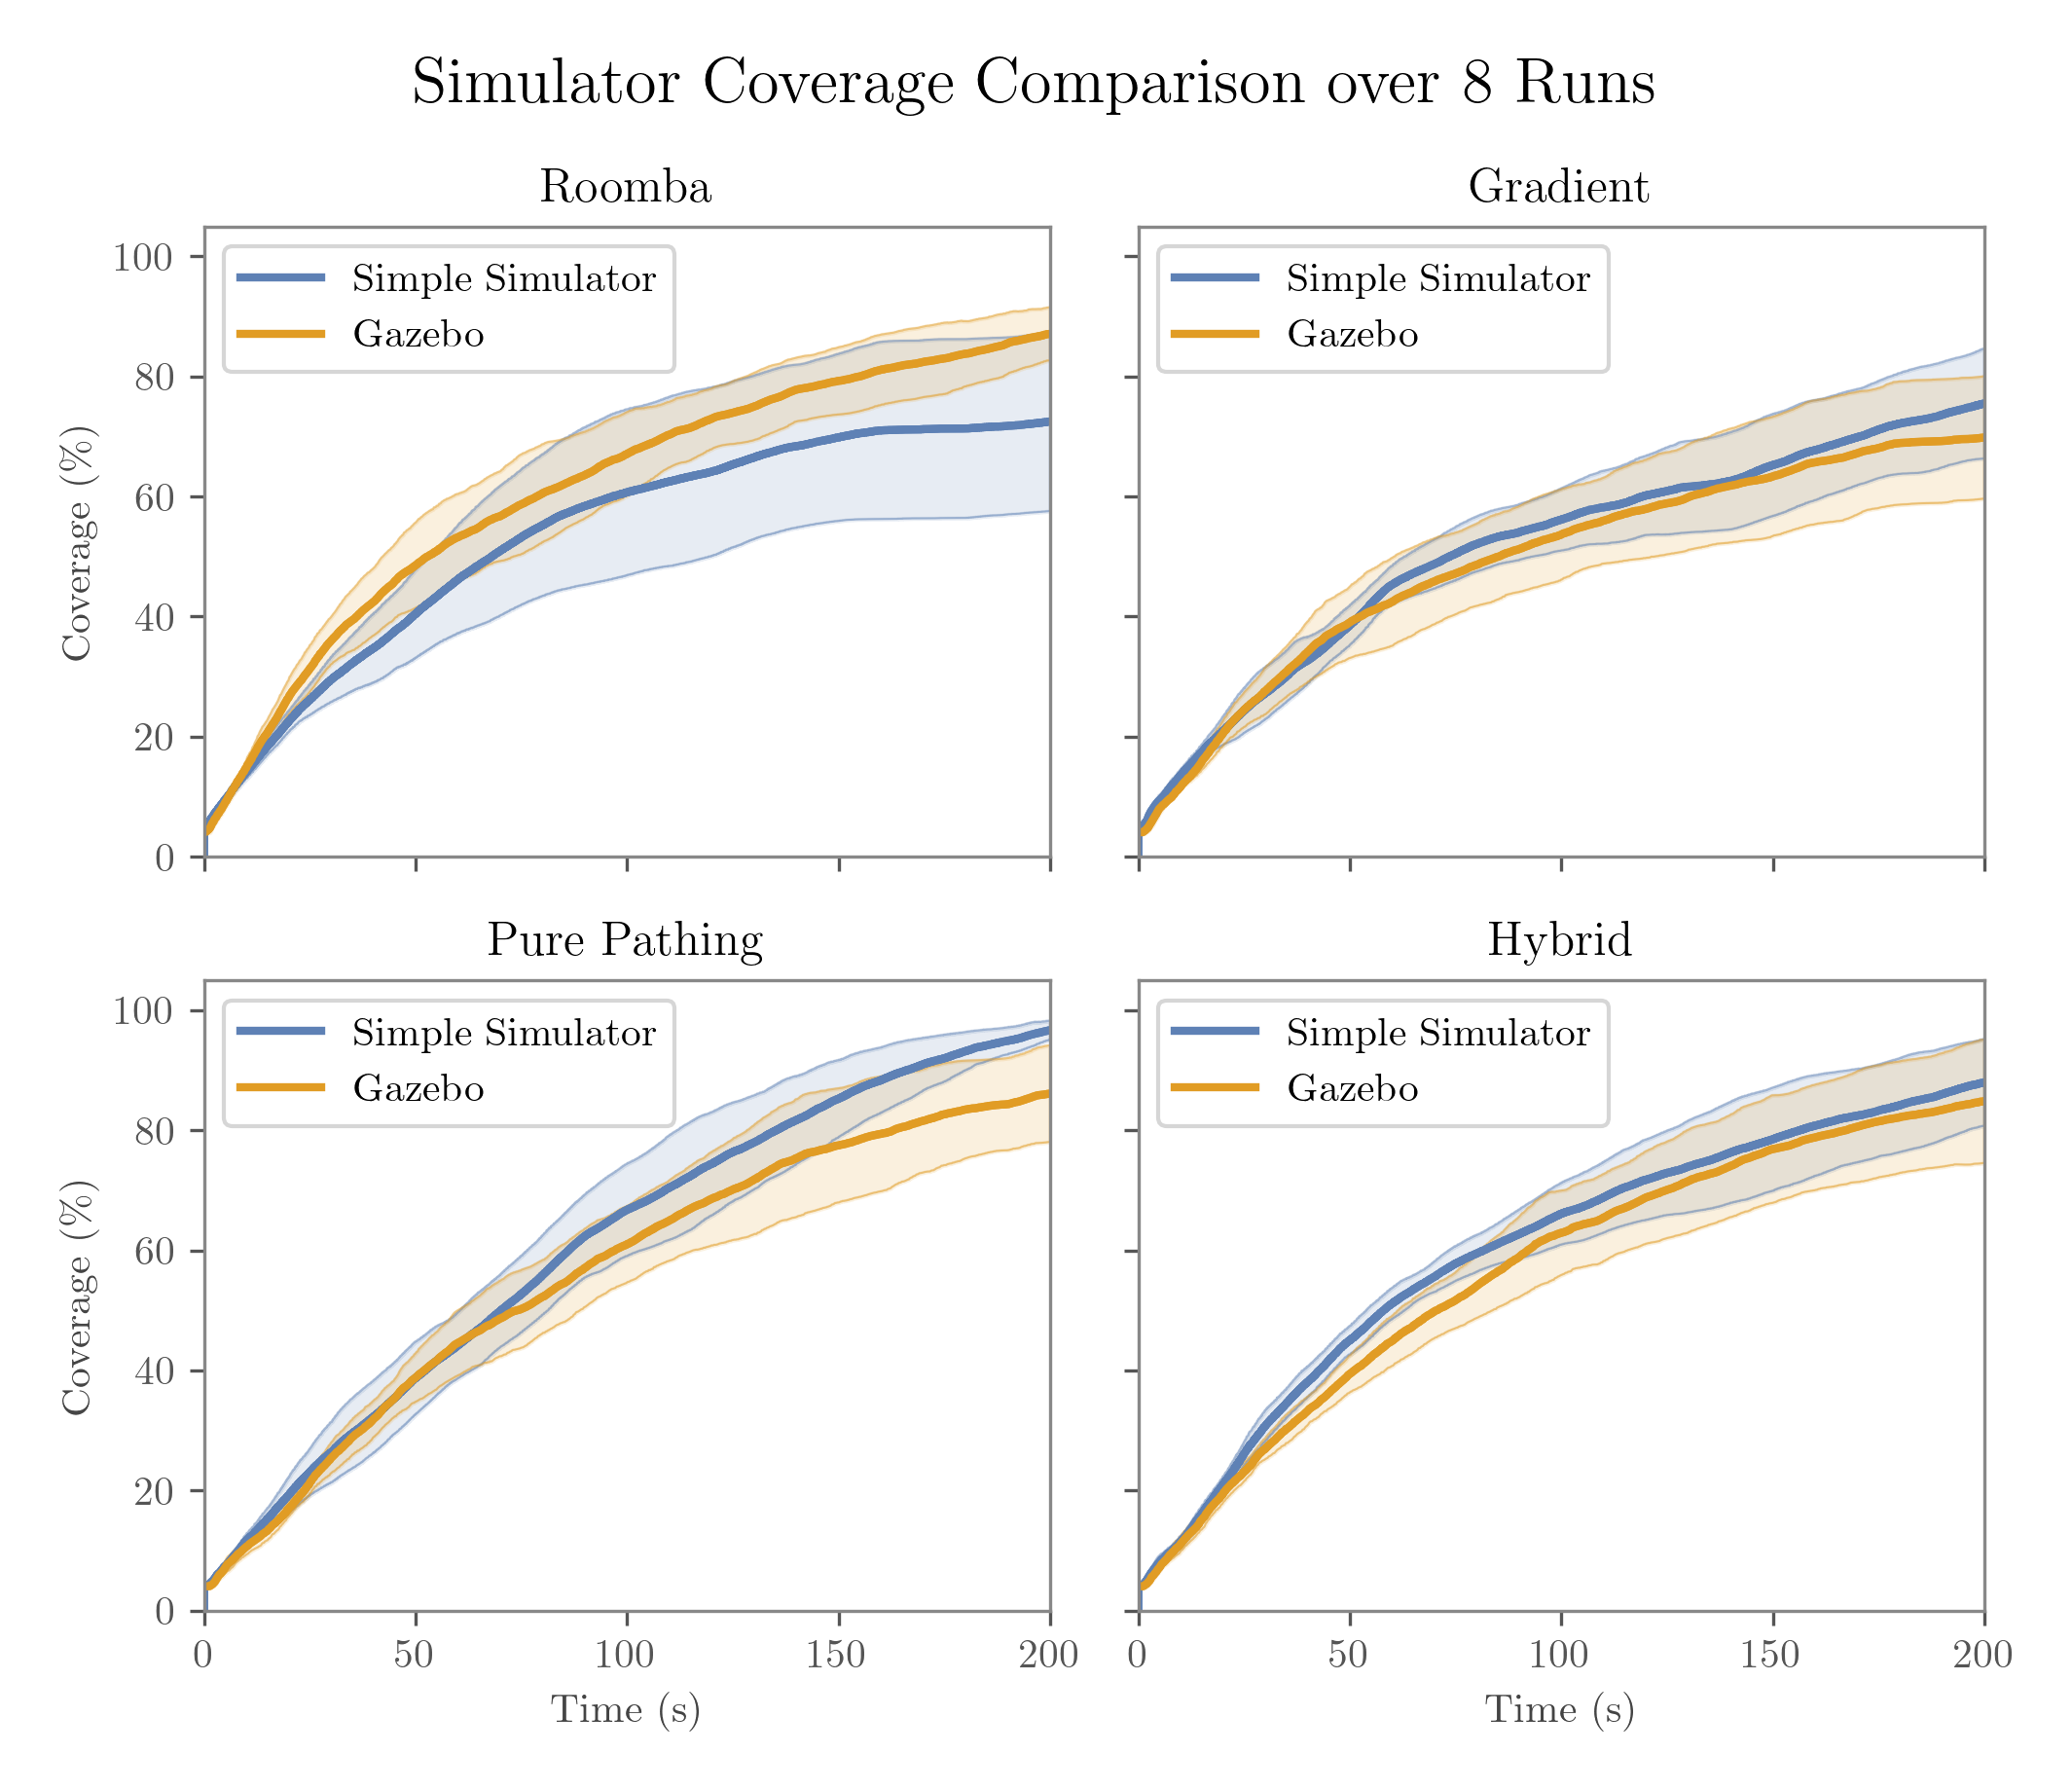
\includegraphics[width=0.95\textwidth]{./figures/plots/consistency/gazebo_vs_simple_sim_coverage.png}
    \end{center}
  \caption{Comparison of coverage over time between ROS 2 Gazebo and \texttt{simple\_sim}.}
  \label{fig:coverage-benchmark-all}
\end{figure}

% TODO: Update this with new
\begin{figure}[H]
    \begin{center}
        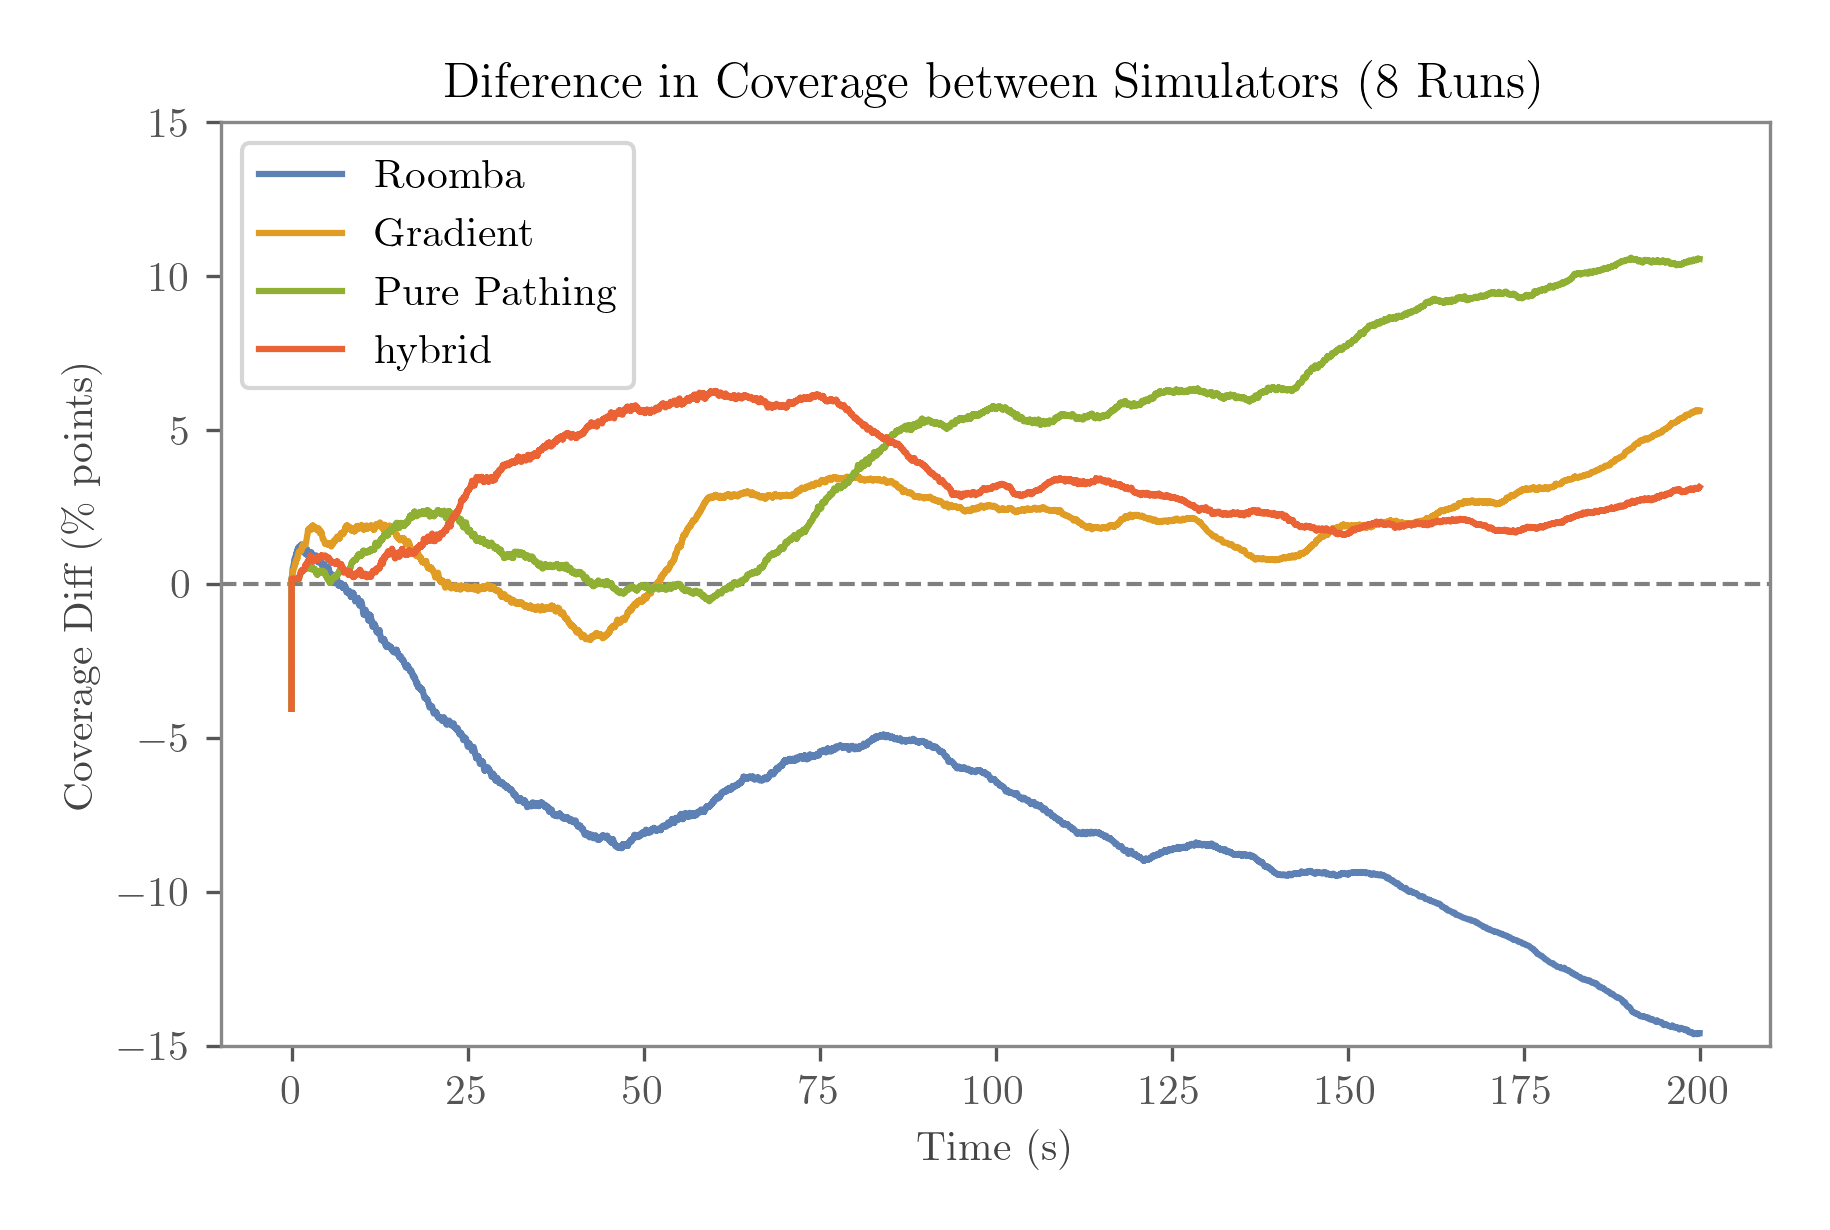
\includegraphics[width=0.95\textwidth]{./figures/plots/consistency/sim_coverage_diff.png}
    \end{center}
    \caption{Comparison of difference in coverage over time between ROS 2 Gazebo and \texttt{simple\_sim}.}
    \label{fig:coverage-benchmark-diff}
\end{figure}

\subsection{Search Algorithm Benchmarks}
Each algorithm was executed across multiple randomly generated maps to evaluate search efficiency. The benchmark shown in \cref{fig:search-coverage-benchmark} presents average coverage over 10 runs, along with minimum and maximum bounds for each time step.

\begin{figure}[H]
    \begin{center}
        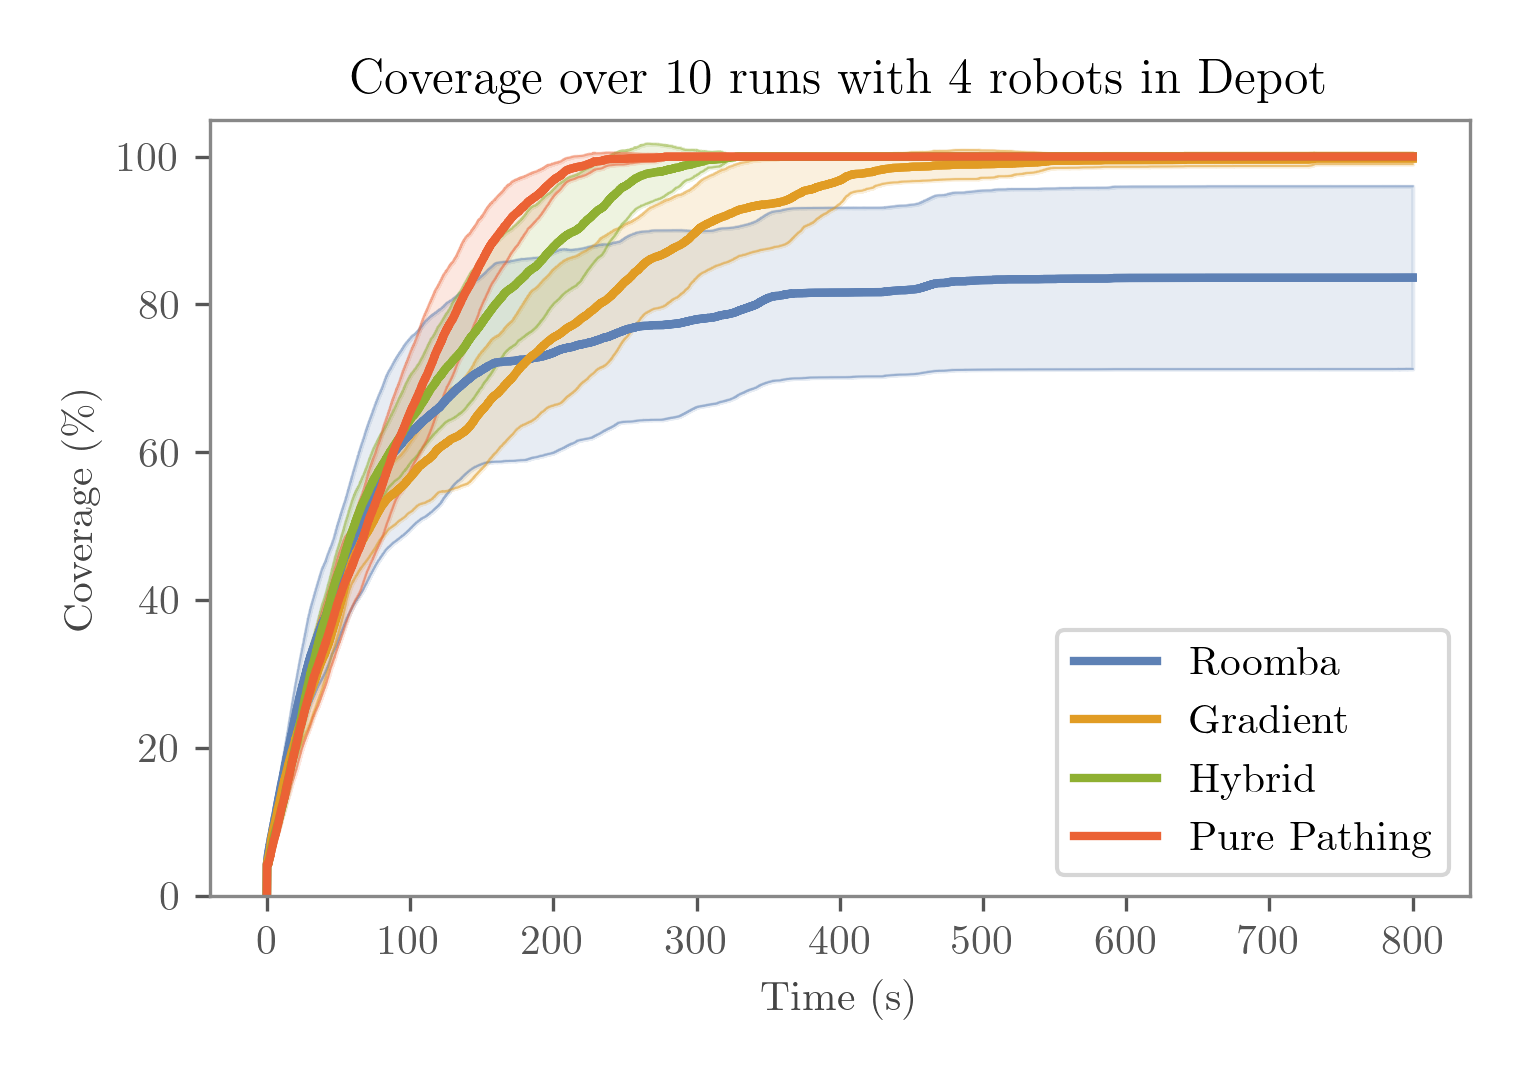
\includegraphics[width=0.95\textwidth]{./figures/plots/benchmarks/coverage-over-10-runs-with-4-robots-in-depot.png}
    \end{center}
    \caption{Coverage performance of search algorithms over 10 runs starting in random positions in the same environment. Shaded regions represent the range between minimum and maximum coverage at each time step.}
    \label{fig:coverage-benchmark}
\end{figure}

All algorithms eventually achieve full coverage, though their exploration efficiency varies significantly. 
Gradient-based methods tend to cover local areas quickly but slow down due to diminishing gradients near fully explored zones. 
Frontier-based methods achieve higher global efficiency by directing robots toward unknown regions, but at a higher computational cost. The hybrid method strikes a balance by switching strategies based on local exploration progress. 
Deep reinforcement learning shows promise but requires further tuning for consistent early-stage performance.

\subsection{Performance}
A critical aspect of the performance of the search algorithms is computational and communication requirement for running the behaviors. 
\subsubsection{Computation Time}
\Cref{fig:computation-performance} presents the computation time distributions for each algorithm running in the same environment.

\begin{itemize}
  \item The \textbf{Roomba} algorithm, being the simplest, exhibits the lowest and most consistent computation time.
\item The \textbf{Pure Pathing} algorithm also performs efficiently on average, though it shows more outliers due to the occasional expensive operations—namely, costmap generation, frontier exploration/evaluation, and path planning—which are not triggered at every time step.
\item The \textbf{Gradient} method is more consistent but slower overall, as gradient recalculation occurs at each step.
\item The \textbf{Hybrid} method was expected to fall between Pure Pathing and Gradient in terms of complexity, and this assumption holds based on the observed data.
\end{itemize}

\begin{figure}[H]
    \begin{center}
        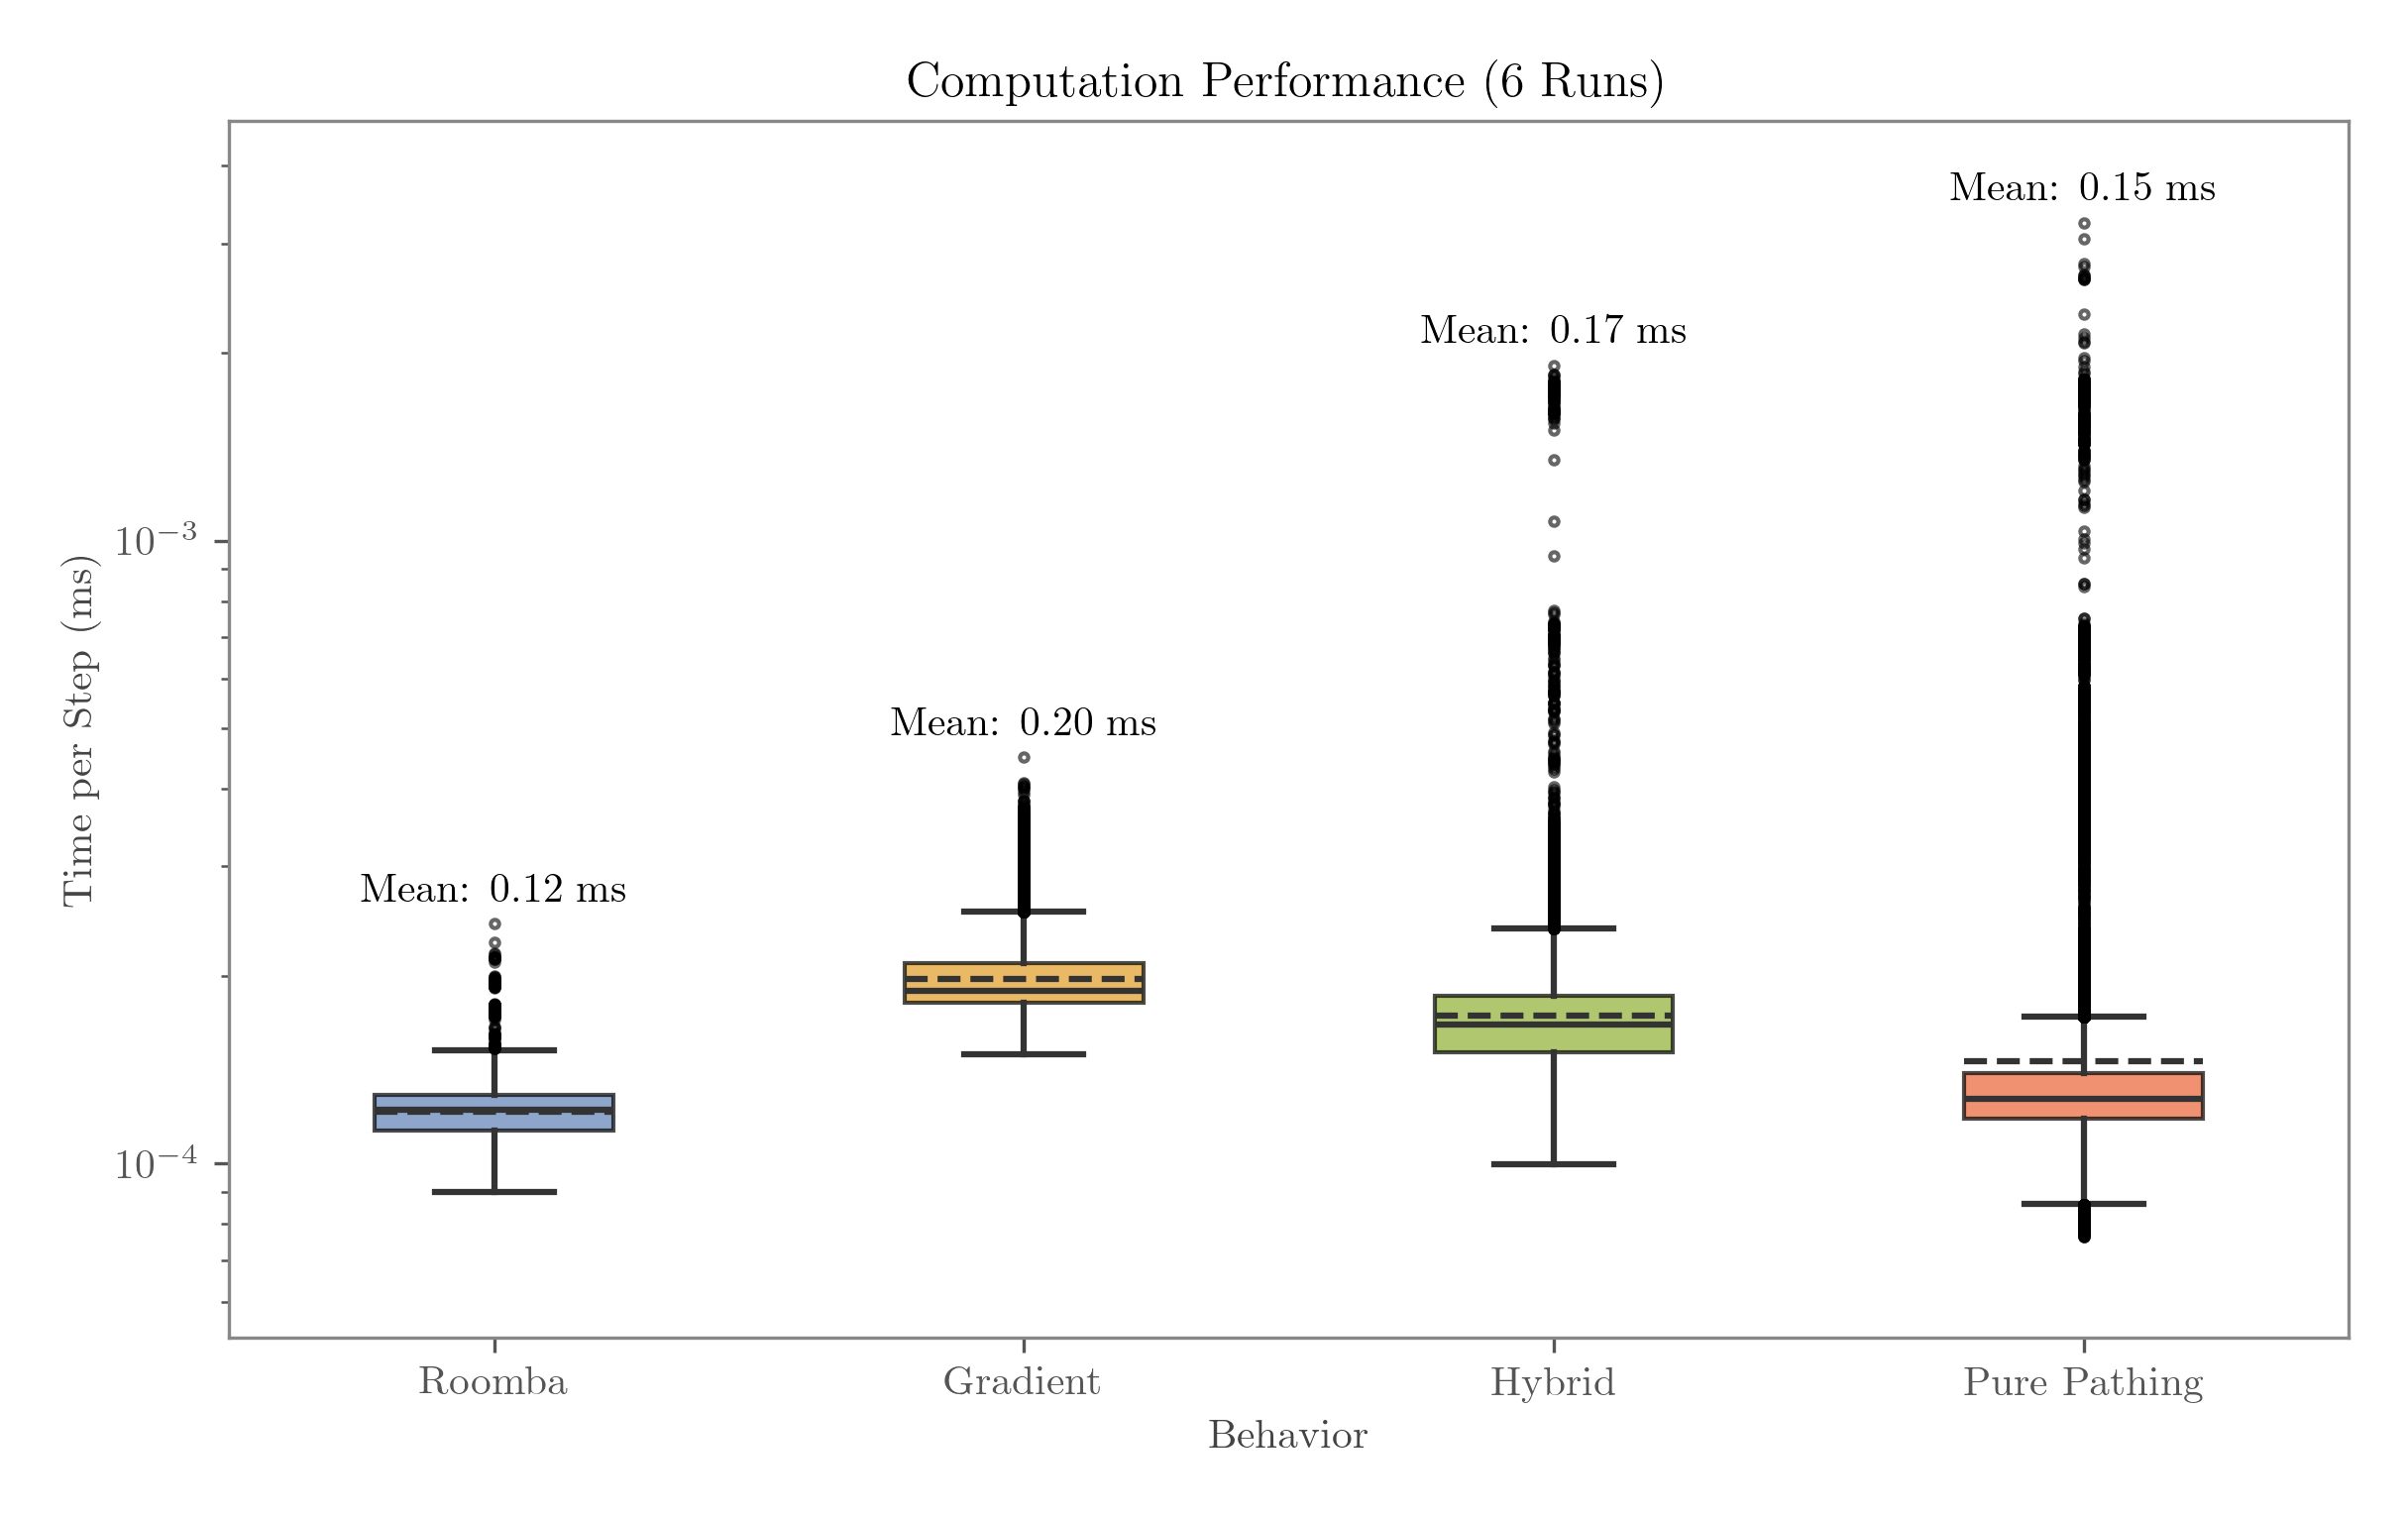
\includegraphics[width=0.95\textwidth]{./figures/plots/computation-performance-(6-runs).png}
    \end{center}
    \caption{Computation time (box plot) for each search algorithm in the same map environment.}
    \label{fig:computation-performance}
\end{figure}

\subsubsection{Communication {\color{red}Load}}
The only messages transmitted during operation are updates to the search grid, which are sent whenever a robot’s internal search grid is modified. From these updates, other robots can synchronize their local search grids and also infer the position of the robot that originated the message.

Each message has a fixed size of 26 bytes. The \texttt{botbrain} library includes a configurable parameter that controls the broadcast frequency, which is set to \SI{10}{Hz} by default. This corresponds to one message every \SI{100}{ms}, resulting in approximately \SI{260}{bytes/sec} of outbound communication per robot.

When compared to the communication technologies considered for real-world deployment (see \cref{sub:communication-methods}), this bandwidth requirement is negligible for most methods, including Wi-Fi, Zigbee, and cellular. However, it may exceed practical limits for LoRa, particularly in multi-robot systems or in scenarios requiring higher message frequencies.

If LoRa is to be considered for deployment, further message compression, reduced transmission frequency, or more aggressive filtering strategies would be necessary to meet the bandwidth constraints.

% TODO: Talk about security. This could make the messages bigger or is this assumed to be handled by the communication protocol?

\subsection{Object Search Performance}
% TODO: How does coverage correlate with the coverage?

